\section{Get Services and Set Transactions}
\label{sec:Services}
Figure~\ref{fig:dfdForAuthServices} illustrates a Data Flow Diagram (DFD) about consuming  
services and set transactions. The Figure shows the scenaries when authentication is or 
not required.


\begin{figure}[bt]
 %\begin{center}
  \centering
    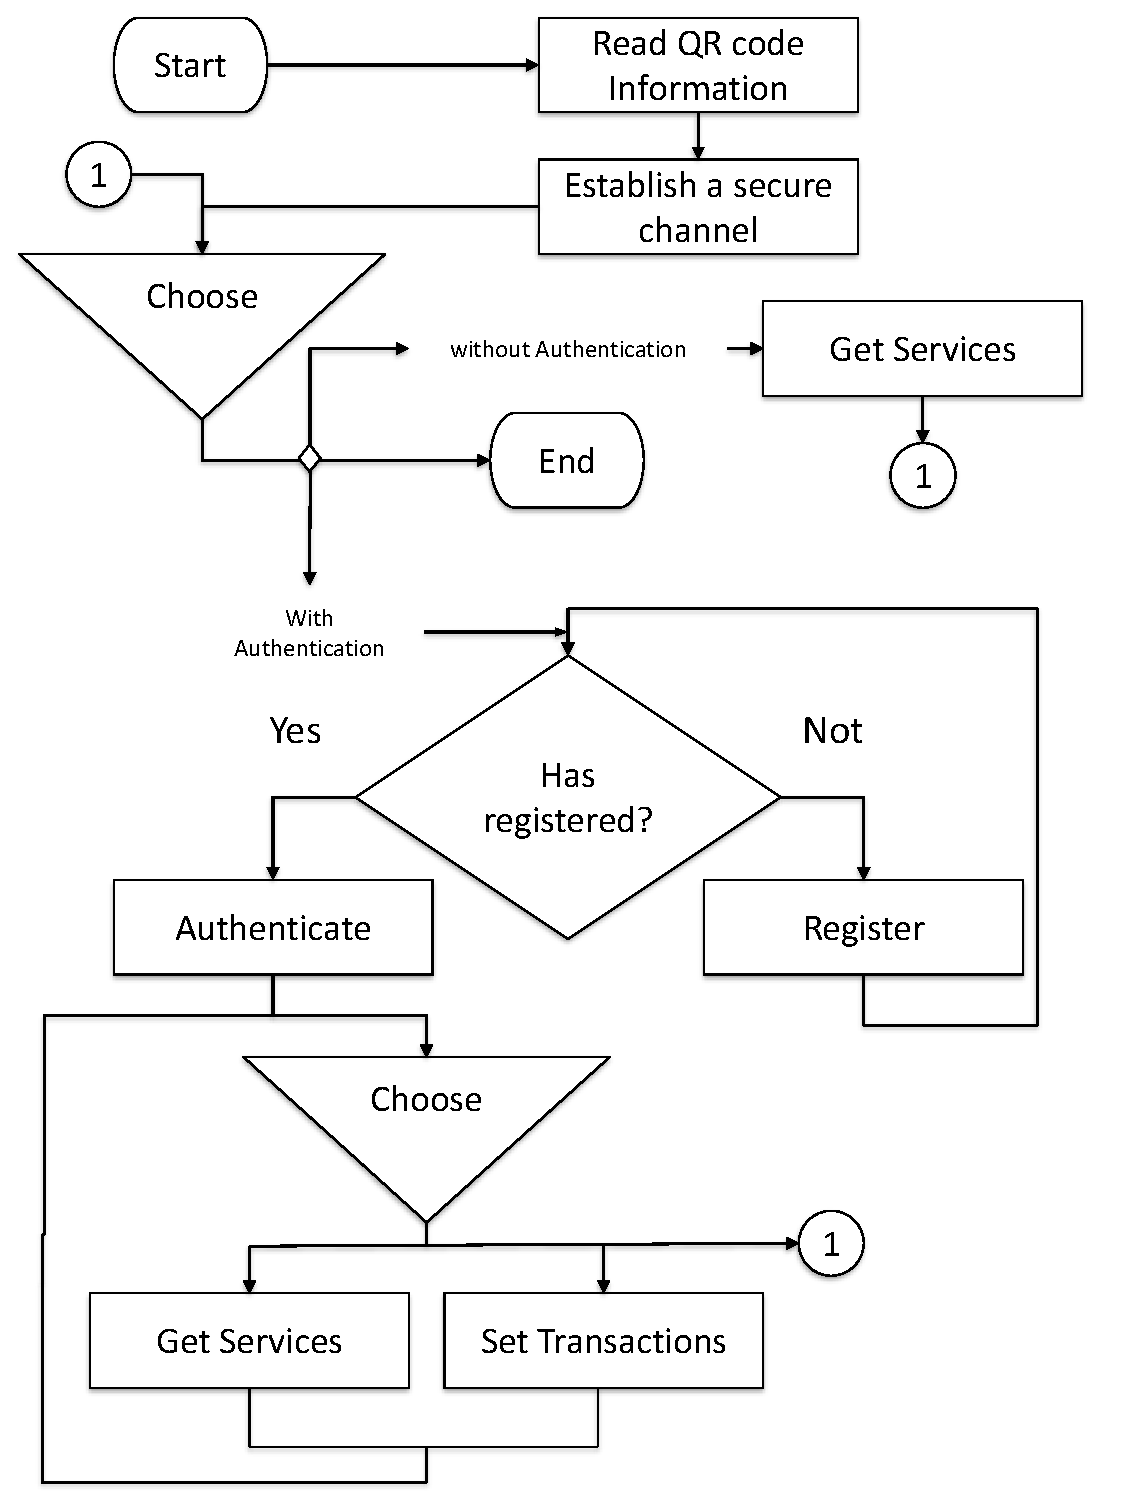
\includegraphics[scale=0.4]{images/dfd.pdf}
        \caption{General DFD about consuming services and set transactions}
    \label{fig:dfdForAuthServices}
 % \end{center}
\end{figure}

\subsection{Getting services without authentication}
\label{ssec:getServNoAuth}

Table~\ref{table:ProtGetServicesNoAuth} describes the process in
Alice and Bob notation, the explanation is as follows:  
\begin{itemize}
  \item  The initial knowledge consists in all values learned by the client and the miner 
        after completed the secure channel stage.
   \item The request of a service consists in sending an identity $C$, the data of the $QR$ code, and a 
        number $n$ denoting the number of service that is requested to be consumed. 
        The client ciphers  these messages using the secret key $K_{C\Server}$ obtained in
        the secure channel stage (see Section~\ref{sec:secureChannel}).
   \item The miner verifies if such a service can be consumed (according permissions) and then, 
        returns the answer $d$; ciphered using, again, the secret key $K_{C\Server}$.
\end{itemize}


\begin{table}[htb]
\footnotesize
\begin{center}
\caption{Get Service Protocol, authentication is not required}
\label{table:ProtGetServicesNoAuth}
\begin{tabular}{|l|}
\hline
           Initial Knowledge                                                             \\
            $C:C\lnk QR \lnk  K_{C\Server}$                                    \\
            $\Server: \Server\lnk K_{C\Server}$    \\ \hline \hline 
           Get a service                                                                        \\
           1.-$\Client\rightarrow \Server: \fat{C \lnk QR \lnk n}_{K_{C\Server}}$          \\ 
           \hspace{5mm} $d=getService(QR,n)$                                  \\  
           2.-$\Server\rightarrow \Client: \fat{C \lnk d}_{K_{C\Server}}$       \\  \hline \hline
\end{tabular}
\end{center}
\end{table}
\normalsize


\subsection{Get Services with authentication}
\label{ssec:ServAuth}
Sometimes it will be necessary to know who is consuming some services; for that, client and
miner are required to be authenticated. The authentication procedure requires a \textit{username} 
and a \textit{password}, which are developed after the \textit{registration process}. 


\subsubsection{Client Registration Process}
\label{sec:Registration}

This part consists in to establish a \textit{username} and a \textit{password}, which
will be mapped with an identity. The \textit{username} must be a valid email and the 
\textit{password} will be created by the user.

Table~\ref{table:reqSessKey} summarizes the protocol
in Alice\&Bob notation, its description is as follows: 
\begin{itemize}
  \item Firstly, the user must establish a secure channel with the miner 
    (see Section~\ref{sec:secureChannel}). In this step all exchanged messages are ciphered 
    using the symmetric key $K_{C\Server}$, which was obtained during the TLS protocol. 
  \item Secondly, the user must generate
    his username and password through the following steps:
    \begin{itemize}
    \item \textbf{First step:} the client sends his username denoted with his email $@$, and  
        a list of personal data $Pd$. 
    \item \textbf{Second step:} the server sends back the user via an email server $\Client_e$ a 
        data obtained of the client's personal information, $Pd$ and a challenge $X=f(Pd)$. 
    \item \textbf{Third step:} then, the client must generate the final password $P$, but
      only the hash is sent, $Hash(P,X)$.  Sending $Hash(P,X)$, we can
      ensure that $P$ will be only known by $\Client$.  
    \end{itemize}
  \item Finally, the miner creates a public and private key for the client ($K_{pub(\Client)}$ 
        and $K_{priv(\Client)}$), which the system maps with the client and the hashed password. 
        Note that, such public and private keys are unknown directly by $\Client$. 
\end{itemize}

\begin{table}[htb]
\footnotesize
\begin{center}
\caption{Client registration process}
\label{table:reqSessKey}
\begin{tabular}{|l|}
\hline
%{\bf Process}                                                                \\\hline\hline
%Initial Knowledge                                                             \\
%$C:N_{C}\lnk K_{pub(S)}\lnk N'_{C} \lnk K'_{CS}$                              \\
%$\ServerW: K_{pub(S)}\lnk K_{priv(S)}\lnk \ServerW\lnk N_{C}\lnk N_{C'}\lnk 
%                      K'_{CS}$                                                \\ \hline \hline
Initial Knowledge                                                             \\
$\Client:K_{C\ServerW}\lnk [@::Pd]$                                                    \\
$\ServerW: K_{C\ServerW}$                                                            \\ \hline \hline
1.-$\Client\rightarrow \ServerW:\fat{[@::Pd]}_{K_{\Client\ServerW}}$                     \\
\hspace{5mm} $X=f(Pd) $                           \\ 
2.-$\ServerW\rightarrow \Client_e: \fat{@\lnk Pd \lnk X}_{K_{\Client_e\ServerW}} $                  \\ 
\hspace{5mm} $\Client$ generates password $P$                          \\  
3.-$\Client\rightarrow \ServerW:\fat{@\lnk Hash(P,X)}_{K_{\Client\ServerW}}$                 \\  
\hspace{5mm} $\ServerW$ generates a pair key ($K_{pub(\Client)}$ and $K_{priv(\Client)}$)\\
\hspace{5mm} $\ServerW$ generates a block $bp = blockPubKey(K_{pub(\Client)})$\\
4.-$\ServerW\rightarrow [\Server_i .. \Server_n]: \fat{\ServerW \lnk bp}_{K_{\Server_i .. \Server_n}}$  \\  
5.-$\ServerW\rightarrow \Client: \fat{C \lnk K_{pub(\Client)}\lnk K_{priv(\Client)}}_{K_{\Server}}$          \\            \hline
New Knowledge Accumulated                                                     \\
$\Client:P\lnk X \lnk K_{pub(\Client)}\lnk K_{priv(\Client)}$                                                                \\
$\ServerW: K_{pub(\Client)}\lnk K_{priv(\Client)}\lnk X \lnk Hash(P,X)\lnk [@::Pd]$       \\\hline \hline 
\end{tabular}
\end{center}
\end{table}
\normalsize




The security properties the protocol must provides are: $P$ to be
known only by $C$; $K_{pub(\Client)}$ and $K_{priv(\Client)}$ to be known by $\Server$; 
and obtain strong authentication between the participants.

% We have verified this protocol using The AVISPA Tool Web
% Interface, available via http://www.avispa-project.org/
% finding the following:
% \begin{itemize}
%     \item The protocol provides secrecy.
%     \item We have proved that the protocol provides
%       \emph{authentication} from the client to the server on message 
%       $f(Pd)$ and \emph{weak authentication} from the server to the
%       client on message $Hash(P)$.
%     \item When we proved \emph{strong authentication}, it failed due
%       to the lack of freshness property generating The Dolev and Yao
%       attacker (of AVISPA tool) a replay attack. However, this attack
%       is already not possible when we consider that $K'_{CS}$ is
%       fresh, which was obtained in an immediately previous step. Even
%       though, we could include timestamps in all steps, however, that
%       is not necessary. 
% \end{itemize}

\subsubsection{Client-Miner Authentication}
\label{ssec:SecAuth}


The authentication process trusts in the users' \textit{username} 
(email) and \textit{password}, so, it is responsibility for the user 
to ensure his secrets. However, it is well known that any system 
cannot trust only in a user and password control access, because of that, 
it is important not only to encrypt the sensible information, but also
to implement more security mechanisms (like authentication procedure) to 
avoid possible attacks.

The goal of this stage is to establish authentication between a client and 
a miner after having a secure tunneling. Table~\ref{table:AuthProtocol} 
describes the authentication part and the explanation is as follows:

\begin{itemize}
  \item Both the client and the miner store all knowledge accumulated
    of previous steps. It is considered to have established a secure tunneling 
    with the miner using the TLS protocol and to have obtained the register
    procedure. So, the initial knowledge of the client consists in to know 
    the session key $K_{\Client\Server}$, his password $P$ and the secret $X$. 
    On the other hand, the miner knows the same session key, the client public and
    private key, personal information of the client, secret $X$ and the hashed 
    $Hash(P,X)$. The following steps are proposed:
    \begin{itemize}
    \item \textbf{First step:} the client sends a challenge to the
      miner $N_\Client$. The miner can map $@$ with $\Client$ and build $hash(@\lnk\Client\Server\lnk N_\Client)$. This message is ciphered with $K_{\Client\Server}$ because the session key has been destined for them. 
    \item \textbf{Second step:} the server responds to the client with a new challenge,
      firstly includes the client name $C$ (which is mapped with $@$) and a hashed message
      composed by $N_{\Client}$ and $X$ both messages must be known by the client. Again,
      all ciphered with $K_{\Client\Server}$.
    \item \textbf{Third step:} Once the client has accepted the previous step, it means that
      he has deduced all previous messages and he has authenticated to the miner, so, the 
      client sends back his username $@$, the challenge response $N_\Client$ as a freshness
      property and his password concatenated with $P$, $X$ and $N_{\Client}$.
  \end{itemize}
\item Finally, after having run the protocol it is expected to obtain strong authentication
    between the client and the miner. 
\end{itemize}
 
\begin{table}[htb]
\footnotesize
\begin{center}
\caption{Authentication Protocol}
\label{table:AuthProtocol}
\begin{tabular}{|l|l|l|}
\hline
{\bf Process}                                                                     \\\hline\hline
            Initial Knowledge                                                     \\
            $\Client:P\lnk X \lnk K_{\Client\Server}$                               \\
            \hspace{5mm}                                                 \\ 
            $\Server: K_{pub(\Client)}\lnk K_{priv(\Client)}\lnk Hash(P,X)\lnk X \lnk[@::Pd] \lnk K_{\Client\Server}$ \\\hline \hline
            Authentication                                                         \\
            1.-$\Client\rightarrow \Server: \fat{\Server \lnk @ \lnk N_{\Client} \lnk 
                                              Hash(@\lnk \Client \lnk \Server \lnk N_\Client)}_{K_{\Client\Server}}$  \\ 
            2.-$\Server\rightarrow \Client: \fat{\Client \lnk hash(N_{\Client},X)}_{K_{\Client\Server}}$ \\ 
            \hspace{5mm} $Y=hash(N_{\Client},hash(P,X))$                          \\              
            3.-$\Client\rightarrow \Server: \fat{@\lnk N_{\Client}\lnk Y}_{K_{\Client\Server}}$            \\ \hline  \hline
            New Knowledge Accumulated                                               \\
            $\Client: \Server \lnk N_\Client \lnk Y$         \\
            \hspace{5mm}                \\ 
            $\Server: \Client  \lnk N_\Client \lnk Y$          \\ 
            \hspace{5mm}                             \\ \hline \hline
\end{tabular}
\end{center}
\end{table}
\normalsize



\subsubsection{Get Services with authentication}
\label{ssec:getServAuth}


\begin{table}[htb]
\footnotesize
\begin{center}
\caption{Get Service Protocol with authentication}
\label{table:ProtGetServicesAuth}
\begin{tabular}{|l|}
\hline
           Initial Knowledge                                                             \\
            $C:C\lnk QR \lnk  K_{C\Server} \lnk Y$                                    \\
            $\Server: \Server\lnk K_{C\Server} \lnk Y$    \\ \hline \hline 
           Get a service                                                                        \\
           1.-$\Client\rightarrow \Server: \fat{C \lnk QR \lnk n \lnk Y}_{K_{C\Server}}$          \\ 
           \hspace{5mm} $d=getService(QR,n)$                                  \\  
           2.-$\Server\rightarrow \Client: \fat{C \lnk d \lnk Y}_{K_{C\Server}}$       \\  \hline \hline
\end{tabular}
\end{center}
\end{table}
\normalsize





\subsection{Set Transactions} 
\label{ssec:setTrans}

As shown by Table~\ref{table:ProtSetTrans} the participants in a transaction 
are the client and a miner.
The client knows the $QR$ code through a scan process with
a car; a secret shared key $K_{\Client\Server}$ established with
a miner in the secure channel process; a proof to have been authenticated
with the miner $N_{\Client\Server}$; and the transaction $T$ that client wish 
to do  (see Table~\ref{table:operations} for types of operations). 
The miner obviously knows also $K_{\Client\Server}$ and $N_{\Client\Server}$. 
\begin{enumerate}
    \item The protocol starts when the client $\Client$ builds the transaction 
        data $t$, the signature of the transaction $\fat{t}_{K_{priv(C)}}$ and sends
        all to the miner $\Server$; all ciphered with the 
        session key $K_{\Client\Server}$.
        The transaction data $t$, using function $setTransaction(\QR,T,N_{\Client\Server})$, 
        is constituted as follows:
        
        \begin{tabular}{lll}
                &               & \\ 
            \{  &               &    \\
                & registered:   & "true" 
                & plate:        & "LVP6598", \\
                & id:           & "1FMYU02Z97KA580G2", \\
                & timestamp:    & "18/09/2018 9:16:34am", \\
                & nonce:         & $N_{\Client\Server}$, \\
                & pubKey:       & $K_{pub(X)}$, \\
                & miner:        & M, \\
                & client:       & C, \\
                & transaction:  & T=$\fat{operation}_{priv(X)}$ \\
            \}  &               &   \\
        \end{tabular}
        
        Both \textit{plate} and \textit{id} are used to identify the car, 
        \textit{timestamp} used to identify the time, $N_{\Client\Server}$
        used to distinguish the session; the public key $K_{pub(X)}$
        of the next owner client, it could be the own $\Client$ or another
        owner;
        \textit{miner} and 
        \textit{client} fields to identify the participants in the transaction; 
        and $T$ stating
        what kind of operation is carrying out (see Table~\ref{table:operations}).
    \item Having the miner accepted the previous message (verifying the  
        session with $N_{\Client\Server}$ and all received messages), he proceeds to build 
        the block $b$ and broadcasts it to all miners $\Server\rightarrow [\Server_i .. \Server_n]$
        in order to execute a mining process; 
        this message is ciphered under \hl{the Ethereum plataform...}
        Block $b$ is as follows:
        \begin{tabular}{lll}
                &               & \\ 
            \{  &               &    \\
                & dataTran:     & t,  \\
                & previousHash: & "000dc75a3...7cf", \\
                & hash:         & "000d20368...1b8",\\
                & blockId:      & 1,\\
                & nonce:        & "42543524",\\
                & timestamp:    & "18/09/2018 9:40:44am" \\
            \}  &               &   \\
        \end{tabular}
        
    \item The miner solving the challenge $\Server_x$, returns again the block, $b'$, 
        but now it is mined. 
    \item Within the \hl{Ethereum Network} there exists a parity node\footnote{
            A parity node is a miner that is close with another and they have usual
            peer to peer communication.
        } to the miner $\Server$
        who also accepts the new block $b'$.
    \item Finally, the miner responds $r$ to the client as a proof that the transaction 
        was carried out successfully.
\end{enumerate}

\begin{table}[htb]
\footnotesize
\begin{center}
\caption{Set Transactions Protocol, authentication required}
\label{table:ProtSetTrans}
\begin{tabular}{|l|}
\hline
           Initial Knowledge                                                             \\
            $C:C\lnk QR \lnk  K_{C\Server} \lnk N_{\Client\Server} \lnk T$               \\
            $\Server: \Server\lnk K_{C\Server} \lnk N_{\Client\Server}$    \\ \hline \hline 
           Set a transaction                                                                        \\
           \hspace{5mm} $t=setTransaction(QR,T,N_{\Client\Server})$                                  \\  
           1.-$\Client\rightarrow \Server: \fat{C \lnk t \lnk \fat{t}_{K_{priv(C)}}}_{K_{C\Server}}$          \\ 
           \hspace{5mm} $b=block(t)$                                  \\  
           2.-$\Server\rightarrow [\Server_i .. \Server_n]: \fat{C \lnk b \lnk N_\Server}_{K_{\Server_i .. \Server_n}}$          \\ 
           \hspace{5mm} $b'=mine(b)$                                  \\  
           3.-$\Server_x\rightarrow [\Server_i .. \Server_n]: \fat{C \lnk b'}_{K_{\Server_i .. \Server_n}}$          \\            
           \hspace{5mm} $r=f(t)$                                  \\  
           4.-$\Server\rightarrow \Client: \fat{C \lnk r \lnk N_{\Client\Server}}_{K_{C\Server}}$       \\  \hline \hline
\end{tabular}
\end{center}
\end{table}
\normalsize
